\normalfalse \difficiletrue \tdifficilefalse
\correctionfalse

%\UPSTIidClasse{11} % 11 sup, 12 spé
%\newcommand{\UPSTIidClasse}{12}

\exer{Pompe à palettes  $\star\star$ \label{B2:12:10}}
\setcounter{numques}{0}
\UPSTIcompetence{B2-12}
\index{Compétence B2-12}
\index{Pompe à palettes}
\ifcorrection
\else
\textbf{Pas de corrigé pour cet exercice.}
\fi

\ifprof
\else
Soit le mécanisme suivant. On a $\vect{AO}=e\vect{i_0}$ et $\vect{AB}=\lambda(t)\vect{i_1}$. De plus $e=\SI{10}{mm}$ et $R=\SI{20}{mm}$. Le contact entre \textbf{0} et \textbf{2} en $B$ est maintenu en permanence (notamment par effet centrifuge lors de la rotation de la pompe).
\begin{center}
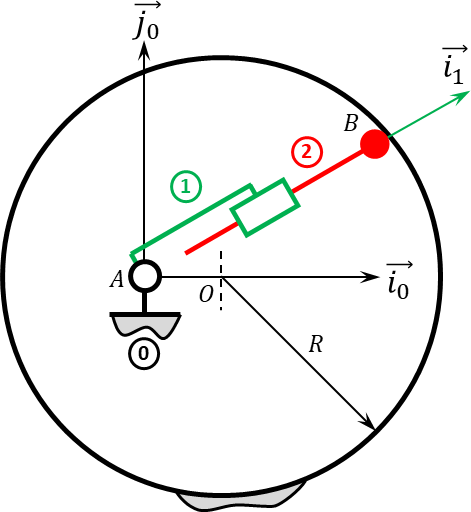
\includegraphics[width=\linewidth]{10_01}
\end{center}
\fi


\question{Tracer le graphe des liaisons.}
\ifprof
\else
\fi


\question{Retracer le schéma cinématique pour $\theta(t)=0 \,\text{rad}$.}
\ifprof
\else
\fi

\question{Retracer le schéma cinématique pour $\theta(t)=\pi\,\text{rad}$.}
\ifprof
\else
\fi


\question{En déduire la course de la pièce \textbf{2}.}
\ifprof
\else
\fi



\ifprof
\else
\begin{flushright}
\footnotesize{Corrigé  voir \ref{B2:12:10}.}
\end{flushright}%
\fi